\documentclass{article}
\usepackage{tikz}
\usepackage{amsmath}
\usetikzlibrary{arrows.meta, positioning, calc}

\begin{document}

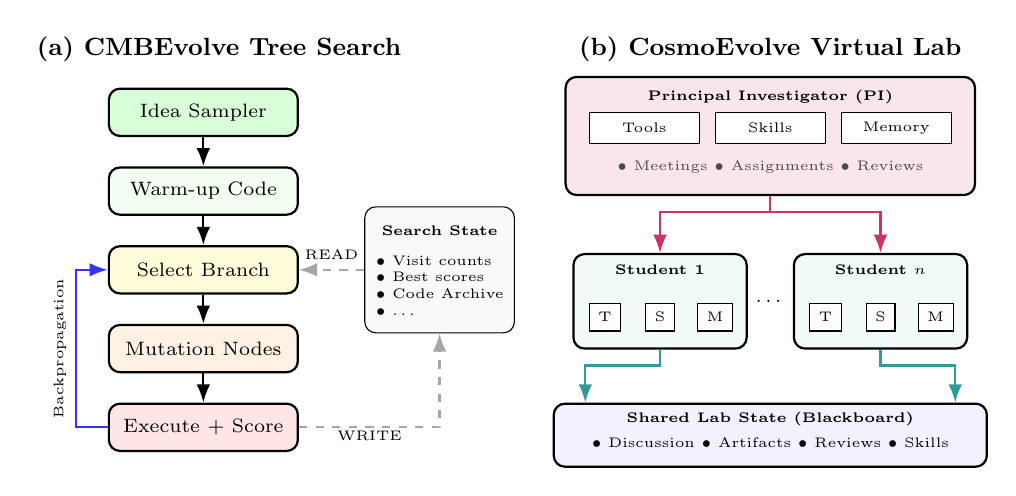
\begin{tikzpicture}[
    >=Latex,
    font=\scriptsize, % Smaller font for compact layout
    every node/.style={align=center},
    box/.style={draw, rounded corners, thick, minimum width=2.4cm, minimum height=0.6cm},
    ideas/.style={box, fill=green!15},
    warmup/.style={box, fill=green!5},
    select/.style={box, fill=yellow!15},
    mutate/.style={box, fill=orange!10},
    eval/.style={box, fill=red!10},
    flow/.style={->, thick},
    backprop/.style={->, thick, color=blue!80},
    stateflow/.style={->, thick, dashed, color=gray!70}
]

% =========================================================
% (a) CMBEvolve
% =========================================================
\node[font=\small\bfseries] (titleA) at (0, 0.8) {(a) CMBEvolve Tree Search};

\node[ideas]  (ideas)  at (-0.2, 0)      {Idea Sampler};
\node[warmup] (warmup) at (-0.2, -1)   {Warm-up Code};
\node[select] (select) at (-0.2, -2)   {Select Branch};
\node[mutate] (mutate) at (-0.2, -3)   {Mutation Nodes};
\node[eval]   (eval)   at (-0.2, -4)   {Execute + Score};

\draw[flow] (ideas) -- (warmup);
\draw[flow] (warmup) -- (select);
\draw[flow] (select) -- (mutate);
\draw[flow] (mutate) -- (eval);

% Precise Backprop Path
\draw[backprop] (eval.west) -- ++(-0.4,0) |- (select.west) 
    node[pos=0.25, rotate=90, anchor=south, color=black, font=\tiny] {Backpropagation};

% Compact Persistent State
\node[draw, rounded corners, fill=gray!5, minimum width=1.9cm, minimum height=1.6cm] (state) at (2.8, -2) {};
\node[font=\tiny\bfseries] at (2.8, -1.5) {Search State};
\node[font=\tiny, align=left] at (2.8, -2.2) {
    $\bullet$ Visit counts\\
    $\bullet$ Best scores\\
    $\bullet$ Code Archive\\
    $\bullet$ \dots
};

% Clean Dash Arrows (No overlap)
\draw[stateflow] (state.west) -- (select.east) 
    node[midway, above, font=\tiny, color=black] {READ};
% WRITE: Move it right 3 points to clear the vertical drop line
\draw[stateflow] (eval.east) -| (state.south) 
    node[pos=0.10, right, font=\tiny, color=black, yshift=-3pt] {WRITE};


% =========================================================
% (b) CosmoEvolve
% =========================================================
\begin{scope}[xshift=7.cm] % Shifting less because of 4cm margins
\node[font=\small\bfseries] (titleB) at (0, 0.8) {(b) CosmoEvolve Virtual Lab};

% PI Agent
\node[draw, thick, fill=purple!10, rounded corners, minimum width=5.2cm, minimum height=1.5cm] (pi) at (0, -0.3) {};
\node[font=\bfseries\tiny] at (0, 0.2) {Principal Investigator (PI)};

% PI Internal
\node[draw, fill=white, font=\tiny, minimum width=1.4cm, minimum height=0.4cm] at (-1.6, -0.2) {Tools};
\node[draw, fill=white, font=\tiny, minimum width=1.4cm, minimum height=0.4cm] at (0, -0.2) {Skills};
\node[draw, fill=white, font=\tiny, minimum width=1.4cm, minimum height=0.4cm] at (1.6, -0.2) {Memory};
\node[font=\tiny, color=black!70] at (0, -0.7) {$\bullet$ Meetings $\bullet$ Assignments $\bullet$ Reviews};

% Student Agents
\foreach \i/\x/\label in {1/-1.4/Student 1, n/1.4/Student $n$} {
    \node[draw, thick, fill=teal!5, rounded corners, minimum width=2.2cm, minimum height=1.2cm] (s\i) at (\x, -2.4) {};
    \node[font=\tiny\bfseries] at (\x, -2.0) {\label};
    
    % Balanced student sub-boxes
    \node[draw, fill=white, font=\tiny, minimum width=0.3cm] at (\x-0.7, -2.6) {T};
    \node[draw, fill=white, font=\tiny, minimum width=0.3cm] at (\x, -2.6) {S};
    \node[draw, fill=white, font=\tiny, minimum width=0.3cm] at (\x+0.7, -2.6) {M};
}
\node at (0, -2.4) {\dots};

% Shared Lab State
\node[draw, thick, fill=blue!5, rounded corners, minimum width=5.5cm, minimum height=0.8cm] (shared) at (0, -4.1) {};
\node[font=\bfseries\tiny] at (0, -3.9) {Shared Lab State (Blackboard)};
\node[font=\tiny] at (0, -4.2) {$\bullet$ Discussion $\bullet$ Artifacts $\bullet$ Reviews $\bullet$ Skills};

% Vertical Connections
\draw[->, thick, color=purple!80] (pi.south) -- ++(0,-0.2) -| (s1.north);
\draw[->, thick, color=purple!80] (pi.south) -- ++(0,-0.2) -| (sn.north);

\draw[->, thick, color=teal!80] (s1.south) -- ++(0,-0.2) -| (shared.170);
\draw[->, thick, color=teal!80] (sn.south) -- ++(0,-0.2) -| (shared.10);

\end{scope}

\end{tikzpicture}

\end{document}